\documentclass[11pt, a4paper]{article}
\usepackage[a4paper, margin=2.5cm]{geometry}

\usepackage[magyar]{babel}

\usepackage{enumitem}
\setlist[itemize]{label=-}
\usepackage{amsmath}

%%% Megjelenítéshez szükséges csomagok %%%
\usepackage[utf8]{inputenc}
\usepackage[T1]{fontenc}
\usepackage{amssymb, amsfonts, amsthm}
\usepackage{xcolor}
\usepackage{tcolorbox}
\tcbuselibrary{theorems,skins,breakable}
\usepackage{tikz}
\usepackage{pgfplots}
\pgfplotsset{compat=1.18}
\usepackage{graphicx}
\usepackage{booktabs}
\usepackage{float}
\usepackage{caption}
\usepackage{microtype}

\usepackage{hyperref}

\begin{document}

\begin{center}
    \LARGE \textbf{Ismétléses permutáció} \\
    \vspace{0.5cm}
\end{center}

\vspace{0.3cm}

\subsection*{1. A lényeg}
Az ismétlés nélküli permutációnál láttuk, hogy ha minden egyes elemünk különböző, akkor $n$ darab dolgot egyszerűen $n!$-féleképpen tudunk sorba rendezni.

De mi történik akkor, ha \textbf{vannak azonos, egymástól megkülönböztethetetlen elemeink is}? Például ha betűkártyákból próbálunk szavakat kirakni, és a betűk között több egyforma is akad (mint az \textit{ALMA} vagy a \textit{MATEMATIKA} szavakban)?

Ha felcserélünk két egyforma betűt vagy golyót egymás között, a sorrend a valóságban \textbf{nem változik meg}: ugyanazt az eredményt látjuk. Az \textbf{ismétléses permutáció} lényege éppen az, hogy az összes lehetséges sorrend ($n!$) számából szisztematikusan \textbf{kiosztjuk a feleslegesen duplán, triplán számolt egyforma eseteket}.

\subsection*{2. Hogyan működik? (A megkülönböztetés gondolatkísérlete)}
Képzeljük el a lehető legegyszerűbb esetet: rakjuk sorba az \textbf{A}, \textbf{A}, \textbf{B} betűket (két darab A és egy darab B betűnk van). Hány különböző 3 betűs szó készíthető belőlük? 

Írjuk fel kézzel az összes létező lehetőséget:
\begin{enumerate}
    \item \textbf{A A B}
    \item \textbf{A B A}
    \item \textbf{B A A}
\end{enumerate}
Összesen pontosan \textbf{3} különböző szót kaptunk. De miért nem $3! = 6$, ahogyan azt az ismétlés nélküli permutációnál megszoktuk?

Játsszuk le a matematikusok kedvenc gondolatkísérletét: \textbf{tegyünk úgy, mintha a két darab A betű mégis megkülönböztethető lenne}, jelöljük őket indexekkel: $A_1$ és $A_2$.

Ekkor a 3 különböző elem ($A_1, A_2, B$) már valóban $3! = 6$-féleképpen állhatna sorba:

\begin{center}
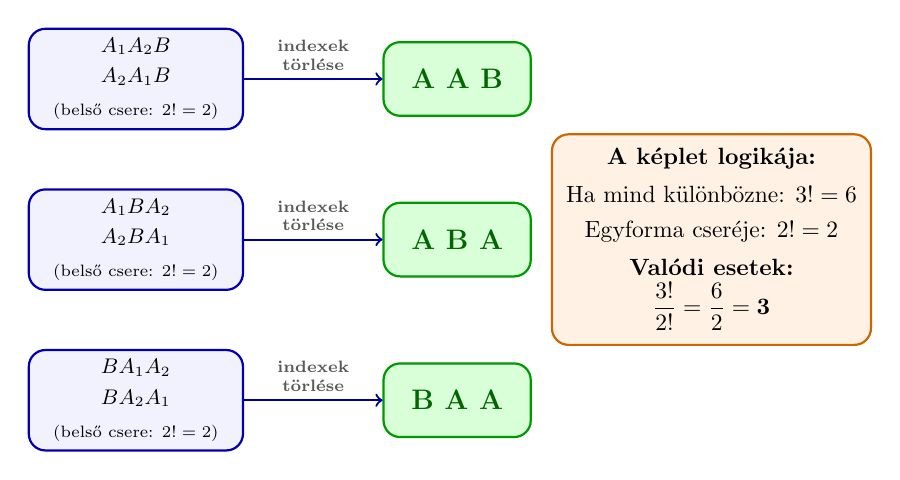
\begin{tikzpicture}[
    scale=0.85, transform shape,
    pairbox/.style={
        draw=blue!70!black,
        fill=blue!5,
        thick,
        rounded corners=6pt,
        minimum width=3.2cm,
        minimum height=1.5cm,
        align=center,
        font=\small
    },
    arrowlabel/.style={
        font=\scriptsize\bfseries,
        text=gray!70!black,
        midway,
        above,
        align=center
    },
    realword/.style={
        draw=green!60!black,
        fill=green!15,
        thick,
        rounded corners=6pt,
        minimum width=2.2cm,
        minimum height=1.1cm,
        align=center,
        font=\large\bfseries,
        text=green!40!black
    }
]
    % 1. oszlop (indexelt esetek)
    \node[pairbox] (p1) at (0, 2.4) {%
        $A_1 A_2 B$\\[2pt]
        $A_2 A_1 B$\\[3pt]
        {\scriptsize(belső csere: $2! = 2$)}
    };

    \node[pairbox] (p2) at (0, 0) {%
        $A_1 B A_2$\\[2pt]
        $A_2 B A_1$\\[3pt]
        {\scriptsize(belső csere: $2! = 2$)}
    };

    \node[pairbox] (p3) at (0, -2.4) {%
        $B A_1 A_2$\\[2pt]
        $B A_2 A_1$\\[3pt]
        {\scriptsize(belső csere: $2! = 2$)}
    };

    % 2. oszlop (valódi szavak)
    \node[realword] (n1) at (4.8, 2.4) {A A B};
    \node[realword] (n2) at (4.8, 0) {A B A};
    \node[realword] (n3) at (4.8, -2.4) {B A A};

    % Nyilak (két sorba törtséggel a tuti olvashatóságért)
    \draw[->, thick, blue!60!black] (p1.east) -- node[arrowlabel] {indexek\\törlése} (n1.west);
    \draw[->, thick, blue!60!black] (p2.east) -- node[arrowlabel] {indexek\\törlése} (n2.west);
    \draw[->, thick, blue!60!black] (p3.east) -- node[arrowlabel] {indexek\\törlése} (n3.west);

    % Összefoglaló doboz jobb oldalon
    \node[draw=orange!80!black, fill=orange!10, thick, rounded corners=6pt, align=center, inner sep=6pt] at (8.6, 0) {%
        \textbf{A képlet logikája:}\\[4pt]
        Ha mind különbözne: $3! = 6$\\[3pt]
        Egyforma cseréje: $2! = 2$\\[4pt]
        \textbf{Valódi esetek:}\\[2pt]
        $\displaystyle \frac{3!}{2!} = \frac{6}{2} = \mathbf{3}$
    };
\end{tikzpicture}
\end{center}

\vspace{0.2cm}
\noindent\textbf{Mi a tanulság?}
Amikor eltüntetjük az indexeket, az $A_1 A_2 B$ és az $A_2 A_1 B$ pontosan ugyanazzá az egyetlen szóvá (AAB) olvad össze. Mivel a 2 darab A betű egymás között $2! = 2$-féleképpen cserélhet helyet, \textbf{minden valódi szóhoz pontosan $2!$ darab fiktív indexelt sorrend tartozott}.

Ezért a helyes darabszámhoz az összes permutációt el kell osztanunk az azonos elemek belső permutációinak számával:
\[
\frac{3!}{2!} = \frac{6}{2} = 3
\]


\vspace{0.3cm}
\noindent\textbf{Egy kicsit összetettebb példa:} \\
Hány különböző anagrammája készíthető a \textbf{PAPAYA} szó betűiből?
\begin{itemize}
    \item \textbf{1. lépés – Leltár:} A szó hossza $n = 6$. A betűk gyakorisága:
    \begin{itemize}
        \item A betű: 3 db
        \item P betű: 2 db
        \item Y betű: 1 db
    \end{itemize}
    \item \textbf{2. lépés – Ellenőrzés:} $3 + 2 + 1 = 6$, tehát az összes betűt felhasználjuk.
    \item \textbf{3. lépés – Képlet alkalmazása:}
    \[
    P_6^{3, 2, 1} = \frac{6!}{3! \cdot 2! \cdot 1!} = \frac{720}{6 \cdot 2 \cdot 1} = \frac{720}{12} = \mathbf{60}
    \]
\end{itemize}
Tehát a PAPAYA betűiből pontosan 60 különböző (értelmes vagy értelmetlen) szó rakható ki.


\subsection*{3. Általános képlet és tulajdonságok}
Tegyük fel, hogy összesen $n$ darab elemet szeretnénk sorba rendezni, de ezek között:
\begin{itemize}
    \item az 1. fajta elemből $k_1$ darab egyforma van,
    \item a 2. fajta elemből $k_2$ darab egyforma van,
    \item \dots
    \item az $r$. fajta elemből $k_r$ darab egyforma van,
\end{itemize}
úgy, hogy az elemek darabszámainak összege kiadja az összes elemet: $k_1 + k_2 + \ldots + k_r = n$.

\vspace{0.2cm}
\noindent\textbf{Definíció és képlet (Ismétléses permutáció)}

$n$ darab elem összes lehetséges sorrendjének számát, ahol az egyes azonos típusú elemek multiplicitása $k_1, k_2, \ldots, k_r$ ($k_1 + \dots + k_r = n$), \textbf{ismétléses permutációnak} nevezzük, és az alábbi képlettel számítjuk ki:
\[
P_n^{k_1, k_2, \ldots, k_r} = \frac{n!}{k_1! \cdot k_2! \cdot \ldots \cdot k_r!}
\]

\vspace{0.2cm}
\noindent\textbf{Fontos észrevétel:}
\begin{itemize}
    \item \textbf{Kapcsolat az ismétlés nélküli permutációval:} Ha minden elem különböző (azaz mindegyikből pontosan $k_i = 1$ darab van), a nevezőben $1! \cdot 1! \dots = 1$ áll, így visszakapjuk a sima $n!$ képletet.
\end{itemize}

\vspace{0.4cm}
\noindent\fbox{
    \begin{minipage}{\dimexpr\textwidth-2\fboxsep-2\fboxrule\relax}
        \vspace{0.2cm}
        \textbf{\large 4. Dolgozat gyorsteszt} \\[0.2cm]
        Amikor a dolgozatban meglátsz egy kombinatorikai feladatot, ellenőrizd ezt a 4 pontot. Ha mindegyik teljesül, akkor ez ismétléses permutáció:
        \begin{enumerate}
            \item \textbf{Minden elemet felhasználunk és sorba rakunk?} (Ugyanannyi a hely, mint az elemek összege: $k_1 + \dots + k_r = n$.) $\rightarrow$ \textbf{IGEN}
            \item \textbf{Számít a sorrend?} (A betűk vagy számjegyek helye eltérő szót/számot eredményez.) $\rightarrow$ \textbf{IGEN}
            \item \textbf{Vannak azonos, egyforma elemek?} (Több egyforma betű, golyó, számjegy vagy lépés van.) $\rightarrow$ \textbf{IGEN}
            \item \textbf{A nevezőbe a csoportok faktoriálisai kerülnek?} (Mindig a darabszámok faktoriálisainak szorzatával osztunk.) $\rightarrow$ \textbf{IGEN}
        \end{enumerate}
        \vspace{0.2cm}
    \end{minipage}
}
\vspace{0.5cm}

\subsection*{5. Tipikus és trükkös feladatok levezetése}

\begin{enumerate}[label=\arabic*., leftmargin=*]
    \item \textbf{Klasszikus anagramma feladat (A „MATEMATIKA” szó)}\\
    \textit{Hány különböző 10 betűs értelmes vagy értelmetlen szó képezhető a MATEMATIKA szó betűinek sorbarendezésével?}
    \begin{itemize}
        \item \textbf{1. lépés – A betűk leltára:} Számoljuk össze gondosan az egyes betűk gyakoriságát:
        \begin{itemize}
            \item M betű: 2 db
            \item A betű: 3 db
            \item T betű: 2 db
            \item E betű: 1 db
            \item I betű: 1 db
            \item K betű: 1 db
        \end{itemize}
        Összes betű: $2 + 3 + 2 + 1 + 1 + 1 = 10$ db.
        \item \textbf{2. lépés – Képlet alkalmazása:}
        \[
        P_{10}^{2, 3, 2, 1, 1, 1} = \frac{10!}{2! \cdot 3! \cdot 2! \cdot 1! \cdot 1! \cdot 1!}
        \]
        \item \textbf{3. lépés – Egyszerűsítés és kiszámítás:}
        \[
        \frac{3\,628\,800}{2 \cdot 6 \cdot 2 \cdot 1 \cdot 1 \cdot 1} = \frac{3\,628\,800}{24} = \mathbf{151\,200}
        \]
        Tehát 151\,200 különböző szó rakható ki.
    \end{itemize}

    \begin{center}
    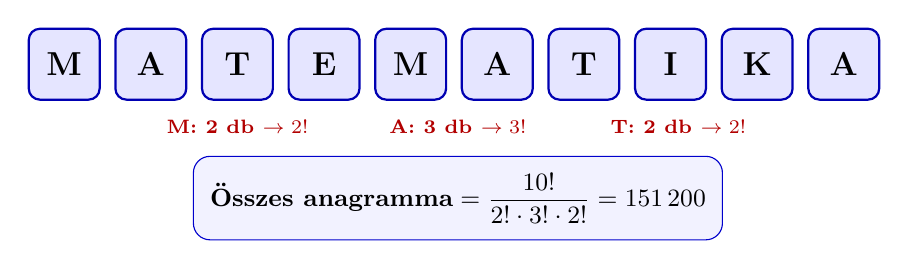
\begin{tikzpicture}[
        letterbox/.style={draw=blue!70!black, fill=blue!10, thick, rounded corners=4pt, minimum size=0.9cm, font=\bfseries\large, align=center},
        countlabel/.style={font=\scriptsize\bfseries, text=red!70!black}
    ]
        \node[letterbox] (m1) at (0,0) {M};
        \node[letterbox] (a1) at (1.1,0) {A};
        \node[letterbox] (t1) at (2.2,0) {T};
        \node[letterbox] (e1) at (3.3,0) {E};
        \node[letterbox] (m2) at (4.4,0) {M};
        \node[letterbox] (a2) at (5.5,0) {A};
        \node[letterbox] (t2) at (6.6,0) {T};
        \node[letterbox] (i1) at (7.7,0) {I};
        \node[letterbox] (k1) at (8.8,0) {K};
        \node[letterbox] (a3) at (9.9,0) {A};

        \node[countlabel] at (2.2,-0.8) {M: 2 db $\rightarrow 2!$};
        \node[countlabel] at (5.0,-0.8) {A: 3 db $\rightarrow 3!$};
        \node[countlabel] at (7.8,-0.8) {T: 2 db $\rightarrow 2!$};

        \node[draw=blue!80!black, fill=blue!5, rounded corners=6pt, inner sep=6pt, font=\small\bfseries] at (5.0,-1.7) {%
            $\displaystyle \text{Összes anagramma} = \frac{10!}{2! \cdot 3! \cdot 2!} = 151\,200$
        };
    \end{tikzpicture}
    \end{center}

    \vspace{0.5cm}

    \item \textbf{A nulla csapdája (Számképzés azonos számjegyekkel)}\\
    \textit{Hány darab 6-jegyű szám készíthető a 0, 2, 2, 3, 3, 3 számjegyek összes lehetséges felhasználásával?}
    \begin{itemize}
        \item \textbf{Vigyázat, kritikus pont:} 6-jegyű szám \textbf{nem kezdődhet 0-val}! Ezért a komplementer elvet használjuk.
        \item \textbf{1. lépés – Összes sorrend megkötés nélkül:}
        Összesen 6 számjegyünk van (1 db 0, 2 db 2-es, 3 db 3-as):
        \[
        \text{Összes} = \frac{6!}{1! \cdot 2! \cdot 3!} = \frac{720}{1 \cdot 2 \cdot 6} = \frac{720}{12} = \mathbf{60}
        \]
        \item \textbf{2. lépés – A tiltott esetek száma (nullával kezdődő sorozatok):}
        Ha az első helyre lefixáljuk a 0-t, a maradék 5 helyre a 2, 2, 3, 3, 3 számjegyeket kell sorba rendeznünk:
        \[
        \text{Tiltott} = \frac{5!}{2! \cdot 3!} = \frac{120}{2 \cdot 6} = \frac{120}{12} = \mathbf{10}
        \]
        \item \textbf{3. lépés – Valódi 6-jegyű számok száma:}
        \[
        \text{Megoldás} = \text{Összes} - \text{Tiltott} = 60 - 10 = \mathbf{50}
        \]
    \end{itemize}

    \begin{center}
    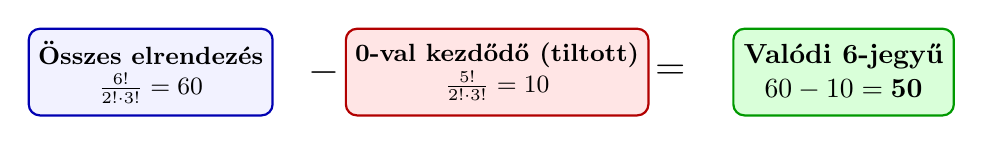
\begin{tikzpicture}[
        statbox/.style={draw=blue!70!black, fill=blue!5, thick, rounded corners=4pt, minimum width=2.8cm, minimum height=1.1cm, align=center, font=\small},
        badbox/.style={draw=red!70!black, fill=red!10, thick, rounded corners=4pt, minimum width=2.8cm, minimum height=1.1cm, align=center, font=\small},
        resbox/.style={draw=green!60!black, fill=green!15, thick, rounded corners=4pt, minimum width=2.8cm, minimum height=1.1cm, align=center, font=\bfseries}
    ]
        \node[statbox] (b1) at (0,0) {\textbf{Összes elrendezés}\\$\frac{6!}{2! \cdot 3!} = 60$};
        \node at (2.2,0) {\Large$-$};
        \node[badbox] (b2) at (4.4,0) {\textbf{0-val kezdődő (tiltott)}\\$\frac{5!}{2! \cdot 3!} = 10$};
        \node at (6.6,0) {\Large$=$};
        \node[resbox] (b3) at (8.8,0) {\textbf{Valódi 6-jegyű}\\$60 - 10 = \mathbf{50}$};
    \end{tikzpicture}
    \end{center}

    \vspace{0.4cm}

    \item \textbf{Rácshálózati utak (A legrövidebb út feladata)}\\
    \textit{Egy rácshálózaton az $A(0,0)$ pontból a $B(4,3)$ pontba szeretnénk eljutni úgy, hogy minden lépésben csak 1 egységet jobbra ($J$) vagy 1 egységet fel ($F$) léphetünk. Hány különböző legrövidebb útvonal létezik?}
    \begin{itemize}
        \item \textbf{A gondolatmenet:} Bármilyen útvonalat is választunk, a cél eléréséhez \textbf{pontosan 4 lépést kell tennünk jobbra ($J$)} és \textbf{pontosan 3 lépést fel ($F$)}.
        \item Minden útvonal leírható egy 7 betűs sorozattal, amely 4 darab $J$ és 3 darab $F$ betűt tartalmaz (például $J J J J F F F$ vagy $J F J F J F J$).
        \item A lehetséges útvonalak száma tehát a 7 betű ismétléses permutációja:
        \[
        P_7^{4, 3} = \frac{7!}{4! \cdot 3!} = \frac{5040}{24 \cdot 6} = \frac{5040}{144} = \mathbf{35}
        \]
    \end{itemize}

    \begin{center}
    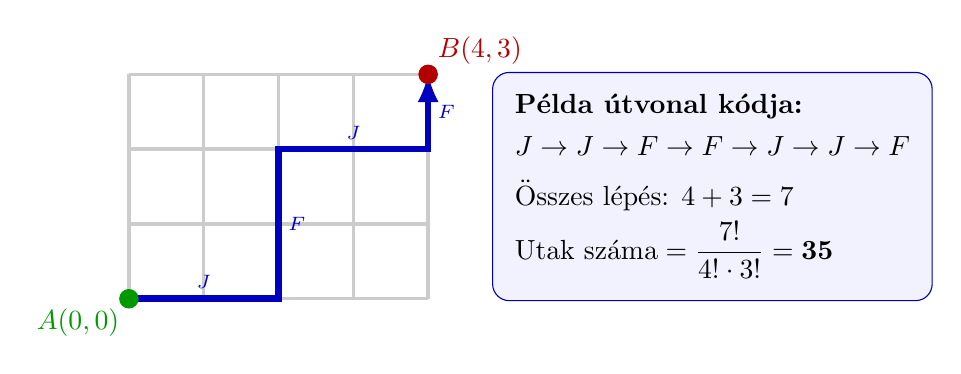
\begin{tikzpicture}[scale=0.95]
        % Rács
        \draw[step=1cm, gray!40, very thick] (0,0) grid (4,3);

        % Példa útvonal vastagon kiemelve
        \draw[line width=2.4pt, blue!75!black, -latex] (0,0) -- (2,0) -- (2,2) -- (4,2) -- (4,3);

        % Kezdő és végpontok
        \filldraw[green!60!black] (0,0) circle (3.5pt) node[below left, font=\bfseries] {$A(0,0)$};
        \filldraw[red!70!black] (4,3) circle (3.5pt) node[above right, font=\bfseries] {$B(4,3)$};

        % Útvonal lépések jelölése
        \node[above, font=\scriptsize\bfseries, text=blue!80!black] at (1,0) {$J$};
        \node[above, font=\scriptsize\bfseries, text=blue!80!black] at (2,0.5) {};
        \node[right, font=\scriptsize\bfseries, text=blue!80!black] at (2,1) {$F$};
        \node[right, font=\scriptsize\bfseries, text=blue!80!black] at (2,2) {};
        \node[above, font=\scriptsize\bfseries, text=blue!80!black] at (3,2) {$J$};
        \node[right, font=\scriptsize\bfseries, text=blue!80!black] at (4,2.5) {$F$};

        % Magyarázó doboz a rács mellett
        \node[draw=blue!70!black, fill=blue!5, rounded corners=6pt, align=left, inner sep=8pt] at (7.8, 1.5) {%
            \textbf{Példa útvonal kódja:}\\[3pt]
            $J \rightarrow J \rightarrow F \rightarrow F \rightarrow J \rightarrow J \rightarrow F$\\[6pt]
            Összes lépés: $4 + 3 = 7$\\[3pt]
            $\displaystyle \text{Utak száma} = \frac{7!}{4! \cdot 3!} = \mathbf{35}$
        };
    \end{tikzpicture}
    \end{center}

    \vspace{0.4cm}

    \item \textbf{Érmefeldobások és bináris kódok}\\
    \textit{Feldobunk egy pénzérmét 8-szor egymás után. Hány olyan dobássorozat létezik, amelyben pontosan 5 fej ($F$) és 3 írás ($I$) szerepel?}
    \begin{itemize}
        \item \textbf{Megoldás:} Olyan 8 elemű sorozatokat keresünk, amelyekben az $F$ betű 5-ször, az $I$ betű 3-szor szerepel.
        \[
        P_8^{5, 3} = \frac{8!}{5! \cdot 3!} = \frac{40\,320}{120 \cdot 6} = \frac{40\,320}{720} = \mathbf{56}
        \]
        Összesen 56 ilyen dobássorozat létezik.
    \end{itemize}

    \vspace{0.5cm}

    \item \textbf{A "ragasztós" trükk ismétléses permutációval}\\
    \textit{A MISSISSIPPI szó betűit úgy rendezzük sorba, hogy a 4 darab S betű mindenképpen egymás mellett maradjon. Hány ilyen szó készíthető?}
    \begin{itemize}
        \item \textbf{1. lépés – Összeragasztás:} A 4 darab S betűt egyetlen "szuper-betűnek" tekintjük: $[SSSS]$.
        \item \textbf{2. lépés – Új betűkészlet meghatározása:}
        \begin{itemize}
            \item M betű: 1 db
            \item I betű: 4 db
            \item P betű: 2 db
            \item $[SSSS]$ blokk: 1 db
        \end{itemize}
        Összesen: $1 + 4 + 2 + 1 = 8$ darab rendezendő elemünk van.
        \item \textbf{3. lépés – Figyelem! Van belső helycsere?}
        Mivel a blokkon belül a 4 darab S betű teljesen egyforma, felcserélésük nem hoz létre új szót ($\frac{4!}{4!} = 1$). Így nincs külön belső szorzó!
        \item \textbf{4. lépés – A végeredmény kiszámítása:}
        \[
        \frac{8!}{1! \cdot 4! \cdot 2! \cdot 1!} = \frac{40\,320}{1 \cdot 24 \cdot 2 \cdot 1} = \frac{40\,320}{48} = \mathbf{840}
        \]
        Tehát pontosan 840 olyan elrendezés van, ahol a négy S betű egymás mellett áll.
    \end{itemize}

    \begin{center}
    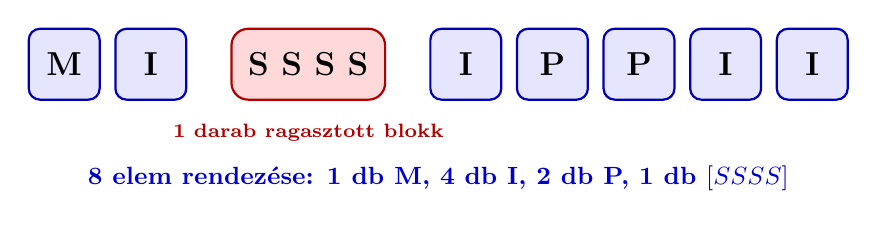
\begin{tikzpicture}[
        elem/.style={draw=blue!70!black, fill=blue!10, thick, rounded corners=4pt, minimum size=0.9cm, font=\bfseries\large},
        block/.style={draw=red!70!black, fill=red!15, thick, rounded corners=6pt, minimum height=0.9cm, font=\bfseries\large, inner sep=6pt}
    ]
        \node[elem] at (0,0) {M};
        \node[elem] at (1.1,0) {I};
        \node[block] at (3.1,0) {S S S S};
        \node[elem] at (5.1,0) {I};
        \node[elem] at (6.2,0) {P};
        \node[elem] at (7.3,0) {P};
        \node[elem] at (8.4,0) {I};
        \node[elem] at (9.5,0) {I};

        \node[below=4pt, font=\scriptsize\bfseries, text=red!70!black] at (3.1,-0.5) {1 darab ragasztott blokk};
        \node[below=16pt, font=\small\bfseries, text=blue!80!black] at (4.75,-0.6) {8 elem rendezése: 1 db M, 4 db I, 2 db P, 1 db $[SSSS]$};
    \end{tikzpicture}
    \end{center}
\end{enumerate}


\end{document}